\documentclass[14pt, a4paper, twoside]{extreport}
\usepackage[utf8]{inputenc}
\usepackage{graphicx}
\usepackage[T2A]{fontenc}
\usepackage{geometry}
\usepackage{array}
\usepackage{graphicx}
\usepackage{setspace}
\usepackage{siunitx}
\usepackage{caption}
\usepackage{titlesec}
\usepackage[russian]{babel}
\usepackage{indentfirst}
\usepackage{setspace}
\usepackage{float}
\usepackage{array}
\usepackage{cellspace}
\usepackage{pgfplots}
\usepackage{pgfplotstable}
\usepackage{tocloft}
\setlength{\cellspacetoplimit}{20pt}
\setlength{\cellspacebottomlimit}{20pt}

\onehalfspacing

\geometry{
  a4paper,
  left=30mm,
  right=20mm,
  top=20mm,
  bottom=20mm
}

\setlength{\parindent}{1.25cm}

\graphicspath{ {images/} }
\captionsetup[figure]{
  labelsep=period,
  justification=centering
}

\renewcommand{\figurename}{Рисунок}
\renewcommand{\contentsname}{Оглавление}

\titleformat{\chapter}[block]{\huge\bfseries\centering}{}{1em}{}
\titleformat{\section}[block]{\normalsize\bfseries}{\thesection}{1em}{}
\titleformat{\subsection}[block]{\normalsize\bfseries}{\thesubsection}{1em}{}
\titlespacing*{\section}{0pt}{\parskip}{-\parskip}
\titlespacing*{\subsection}{0pt}{\parskip}{-\parskip}
\titlespacing{\chapter}{0pt}{0pt}{0pt}

\renewcommand{\cftbeforetoctitleskip}{-30pt}
\renewcommand{\cftaftertoctitleskip}{-10pt}

\begin{document}
\begin{titlepage}
  \begin{center}
    \small
    \underline{
      \begin{minipage}{0.2\textwidth}
        \centering
        
\includegraphics[width=3cm]{BMSTU logo}
      \end{minipage}
      \hfill
      \begin{minipage}{0.8\textwidth}
        \begin{center}

          \textbf{Министерство науки и высшего образования Российской Федерации
            Федеральное государственное бюджетное образовательное учреждение высшего образования «Московский государственный технический университет имени Н.Э. Баумана национальный исследовательский университет»
          (МГТУ им. Н.Э. Баумана)}
        \end{center}
      \end{minipage}

    }

    \vspace{7cm}
    \Large
    \textbf{Лабораторная работа Э-113} \\
    "Определение емкости конденсатора по осциллограмме его разряда через резистор"\\
    \vspace{5cm}
    \normalsize
    \begin{tabular}{p{8cm}p{6cm}}
      \textbf{Студент группы ИУ1-31Б} & \hrulefill \\
      & «\underline{\hspace{1.5cm}}»\underline{\hspace{2.5cm}}2025 г. \\
      & \\
      \textbf{Преподаватель} & \hrulefill \\
      & «\underline{\hspace{1.5cm}}»\underline{\hspace{2.5cm}}2025 г. \\
    \end{tabular}
    \vfill{\Large{Москва, 2025}}
  \end{center}
\end{titlepage}

\tableofcontents
\newpage

\chapter{Конспект}
\section{Цели и задачи работы}
\textbf{Цель работы} - экспериментальное изучение законов электростатики, в частности, раздела «Проводники в электрическом поле».

\textbf{Задачи работы} - изучение процесса разряда конденсатора, измерение постоянной времени цепи и емкости конденсатора. Приобретение навыков работы с электроаппаратурой и электроизмерительными приборами.

\section{Оборудование}
Лабораторный стенд (\ref{fig:scheme}) - схема на магнитной основе, собираемая из пластиковых монтажных элементов, включая сопротивления, емкость, источник ЭДС, кнопки-выключатели для замыкания цепи и монтажные перемычки.
К приборам и принадлежностям относятся также компьютер с необходимым программным обеспечением, осциллографический датчик напряжения для регистрации электрической разности потенциалов на активном сопротивлении и соединительный кабель для подключения датчика к компьютеру.
\begin{figure}[H]
  \centering
  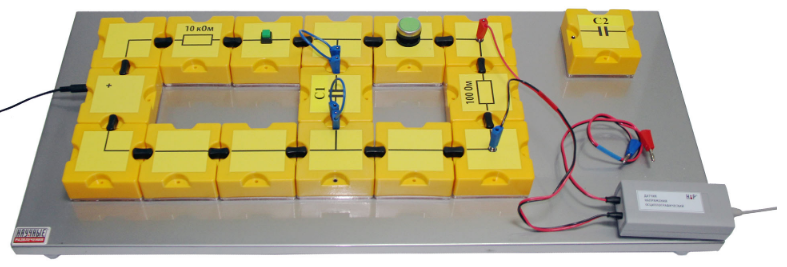
\includegraphics[width=\textwidth]{scheme}
  \caption{}
  \label{fig:scheme}
\end{figure}

\section{Теоретическая часть}
При разрядке конденсатора на резистор в отсутствии источника ЭДС  в контуре сумма падений напряжений равна нулю.
\begin{equation}
  U_C+U_R = 0
  \label{eq:tensionSum}
\end{equation}

Учитывая очевидные соотношения:
\begin{equation}
  U_c = \frac{q}{C},\text{ } q = \int\limits_{0}^{t} Idt,\text{ } U_R = IR
  \label{eq:default}
\end{equation}

Можно получить следующее уравнение
\begin{equation}
  \frac{1}{C}\int\limits_{0}^{t} Idt + IR = 0
  \label{eq:tensionSumUpdated}
\end{equation}
где R - сопротивление резистора, I - ток в цепи, C - емкость конденсатора, q - заряд на обкладках конденсатора.

Продифференцировав данное уравнение по времени и пронормировав его, получим:
\begin{equation}
  \frac{dI}{dt} + \frac{1}{RC}I = 0
  \label{eq:diffEquation}
\end{equation}

Это уравнение будет иметь следующие решения:
\begin{equation}
  I = I_0e^\frac{t}{RC} = I_0e^\frac{t}{\tau}
  \label{eq:solutions}
\end{equation}

В  этом уравнении введена замена $\tau = RC $ - постоянная времени разрядки конденсатора или интервал времени за которое начальный ток $I_0$ уменьшится в $e$ раз.

Тогда изменение заряда в интервале времени ($t_1$, $t_2$) будет иметь вид
\begin{equation}
  \Delta q = \int\limits_{t_1}^{t_2} Idt
\end{equation}

Зная падение напряжения на резисторе(по модулю оно равно падению напряжения на конденсаторе) в эти моменты, емкость конденсатора найдем из закона пропорциональности заряда падению напряжения.
\begin{equation}
  C = \frac{\Delta q}{\Delta U} = \frac{\int\limits_{t_1}{t_2} Idt}{U_1-U_2}
  \label{eq:capacity}
\end{equation}

Другой способ измерения емкости конденсатора основан на знании времени разрядки конденсатора и сопротивления резистора. Измеряя по осциллограмме время $\tau$, в течение которого сила тока $I_0$ на конденсаторе становится меньше в $e$ раз , вычисляем емкость конденсатора по формуле:
\begin{equation}
  C = \frac{\tau}{R}
  \label{eq:capacityFromTime}
\end{equation}

\begin{figure}[H]
  \centering
  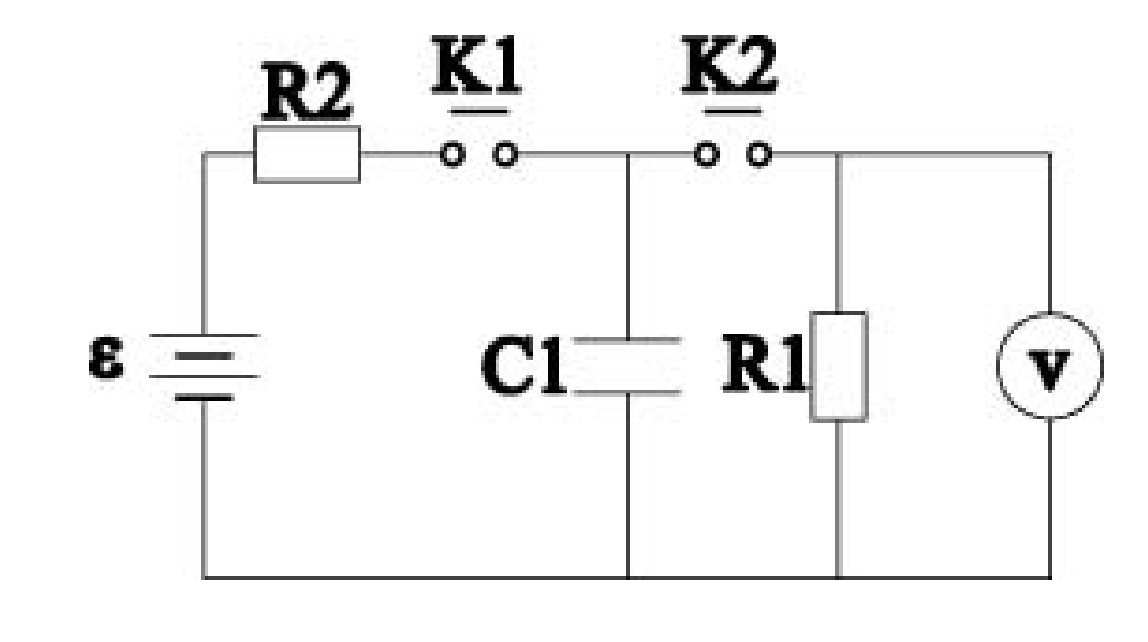
\includegraphics[width=0.8\textwidth]{circuit}
  \caption{Схема для измерения емкости конденсатора}
  \label{}
\end{figure}
\section{Лабораторная установка}

В состав лабораторной установки входят элементы, собранные в схему для исследования разрядки конденсатора. Для замыкания цепи зарядки конденсатора и для осуществления его разряда через резистор используются кнопки-выключатели без фиксации. Соединение элементов электрических цепей производится с помощью монтажных перемычек, а также с помощью гибких проводов со штекерными разъемами, которые применяются для включения в цепь элементов, варьируемых в ходе опыта. Ряд элементов схемы имеют на верхней поверхности гнезда для подключения штекеров, например, для присоединения измерительного кабеля осциллографического датчика напряжения к активному сопротивлению.

\chapter{Выполнение работы}

В результате измерений были получены значения представленные в приложениях \ref{chap:C1} (конденсатор 1) и \ref{chap:C2} (конденсатор 1).

\section{Конденсатор 1}
Погрешность измерений для малого количества измерений(5):

$\Delta C_1 = t_\text{P, f} \sqrt{\frac{\sum_{i=1}^{n} (x_i - \tilde{x})^2}{n(n-1)}}$

Для нашей работы выберем $t_\text{P, f} = 2.57 $.

\subsection{Вычисление электроемкости через заряд }
Среднее значение емкости полученное в результате измерений :

$ \tilde{C_{11}} = \frac{1}{n}\sum_{i=1}^{n} C_\text{1i} = 4,89 \text{ мкФ} $

$\Delta C_{11} = 2.57 \sqrt{\frac{0,0019}{5(5-1)}} = 0,025 \text{ мкФ}$

Получаем следующее значение
\begin{center}
  $C_{11} = 4,89 \pm 0,025 \text{ мкФ}$
\end{center}

\subsection{Вычисление электроемкости через заряд }

Среднее значение емкости полученное в результате измерений :

$ \tilde{C_{12}} = \frac{1}{n}\sum_{i=1}^{n} C_\text{1i} = 4,48 \text{ мкФ} $

$\Delta C_{12} = 2.57 \sqrt{\frac{0,268}{5(5-1)}} = 0,297 \text{ мкФ}$

Получаем следующее значение
\begin{center}
  $C_{11} = 4,48 \pm 0,297 \text{ мкФ}$
\end{center}
\section{Конденсатор 2}

$\Delta C_2 = t_\text{P, f} \sqrt{\frac{\sum_{i=1}^{n} (x_i - \tilde{x})^2}{n(n-1)}}$

Для нашей работы выберем $t_\text{P, f} = 2.57 $.

\subsection{Вычисление электроемкости через заряд }
Среднее значение емкости полученное в результате измерений :

$ \tilde{C_{21}} = \frac{1}{n}\sum_{i=1}^{n} C_\text{1i} = 1,20 \text{ мкФ} $

$\Delta C_{21} = 2.57 \sqrt{\frac{0,002}{5(5-1)}} = 0,030 \text{ мкФ}$

Получаем следующее значение
\begin{center}
  $C_{11} = 1,20 \pm 0,030 \text{ мкФ}$
\end{center}

\subsection{Вычисление электроемкости через заряд }

Среднее значение емкости полученное в результате измерений :

$ \tilde{C_{22}} = \frac{1}{n}\sum_{i=1}^{n} C_\text{1i} = 1,08 \text{ мкФ} $

$\Delta C_{22} = 2.57 \sqrt{\frac{0,008}{5(5-1)}} = 0,051 \text{ мкФ}$
Получаем следующее значение
\begin{center}
  $C_{11} = 1,08 \pm 0,051 \text{ мкФ}$
\end{center}
\section{Вывод}

По результатм проведенных измерений и вычислений можно сделать вывод о том, что измерение электроемкости через заряд на конденсаторе позволяет добиться большей точности.
\chapter{Контрольные вопросы}
\section{Электроёмкость}
Электроёмкость $C$ определяется как отношение заряда $q$, накопленного на обкладках, к напряжению $U$ между ними:
\[
  C = \frac{q}{U}.
\]

\section{Ёмкость плоского конденсатора}
Для плоского конденсатора с площадью пластин $S$, расстоянием между ними $d$ и диэлектрической проницаемостью $\varepsilon = \varepsilon_0 \varepsilon_r$:
\[
  C = \frac{\varepsilon_0 \varepsilon_r S}{d}.
\]

\section{Время разряда конденсатора}
Время разряда определяется \textit{постоянной времени} $\tau = RC$. Именно она задаёт скорость экспоненциального спада напряжения и тока.

\section{Постоянная времени цепи}
\[
  \tau = RC.
\]
Это время, за которое напряжение (или ток) уменьшается в $e \approx 2.718$ раза.

\section{Уравнение напряжения при разряде}
Дифференциальное уравнение:
\[
  R \frac{dq}{dt} + \frac{q}{C} = 0 \quad \Rightarrow \quad q(t) = q_0 e^{-t/(RC)}.
\]
Тогда напряжение на конденсаторе:
\[
  U(t) = U_0 e^{-t/(RC)}.
\]

\section{Энергия заряженного конденсатора}
Энергия определяется выражением:
\[
  W = \frac{1}{2} C U^2 = \frac{q^2}{2C} = \frac{1}{2} qU.
\]

\section{Зависимость быстроты разряда}
Характер быстроты разряда задаётся величиной $RC$:
\[
  \tau = RC.
\]
При увеличении $C$ или $R$ разряд идёт медленнее; при их уменьшении~--- быстрее. Таким образом, быстрота разряда обратно пропорциональна произведению $RC$.

\appendix

\titleformat{\chapter}[block]{\huge\bfseries\centering}{}{0pt}{}

\chapter{Приложение}
\label{chap:C1}
\begin{table}[H]
  \centering
  \resizebox{\textwidth}{!}{%
    \begin{tabular}{llllllll}
      \hline
      \multicolumn{1}{|l|}{\textbf{}}  & \multicolumn{1}{l|}{\textbf{U1, В}} & \multicolumn{1}{l|}{\textbf{U2, В}} & \multicolumn{1}{l|}{\textbf{Q, Кл}} & \multicolumn{1}{l|}{\textbf{C, мкФ}} & \multicolumn{1}{l|}{\textbf{t1, мс}} & \multicolumn{1}{l|}{\textbf{t2,мс}} & \multicolumn{1}{l|}{\textbf{C=(t2-t1)/R, мкФ}} \\ \hline
      \multicolumn{1}{|l|}{\textbf{1}} & \multicolumn{1}{l|}{2,71}           & \multicolumn{1}{l|}{0,09}           & \multicolumn{1}{l|}{12,90}          & \multicolumn{1}{l|}{4,92}          & \multicolumn{1}{l|}{0,01}            & \multicolumn{1}{l|}{0,47}           & \multicolumn{1}{l|}{4,60}                    \\ \hline
      \multicolumn{1}{|l|}{\textbf{2}} & \multicolumn{1}{l|}{2,75}           & \multicolumn{1}{l|}{0,10}           & \multicolumn{1}{l|}{12,90}          & \multicolumn{1}{l|}{4,87}          & \multicolumn{1}{l|}{0,01}            & \multicolumn{1}{l|}{0,42}           & \multicolumn{1}{l|}{4,10}                    \\ \hline
      \multicolumn{1}{|l|}{\textbf{3}} & \multicolumn{1}{l|}{2,74}           & \multicolumn{1}{l|}{0,11}           & \multicolumn{1}{l|}{12,90}          & \multicolumn{1}{l|}{4,90}          & \multicolumn{1}{l|}{0,01}            & \multicolumn{1}{l|}{0,45}           & \multicolumn{1}{l|}{4,40}                    \\ \hline
      \multicolumn{1}{|l|}{\textbf{4}} & \multicolumn{1}{l|}{2,74}           & \multicolumn{1}{l|}{0,09}           & \multicolumn{1}{l|}{12,90}          & \multicolumn{1}{l|}{4,87}          & \multicolumn{1}{l|}{0,01}            & \multicolumn{1}{l|}{0,46}           & \multicolumn{1}{l|}{4,50}                    \\ \hline
      \multicolumn{1}{|l|}{\textbf{5}} & \multicolumn{1}{l|}{2,72}           & \multicolumn{1}{l|}{0,12}           & \multicolumn{1}{l|}{12,70}          & \multicolumn{1}{l|}{4,88}          & \multicolumn{1}{l|}{0,01}            & \multicolumn{1}{l|}{0,49}           & \multicolumn{1}{l|}{4,80}                    \\ \hline
      \multicolumn{1}{|l|}{}           & \multicolumn{1}{l|}{}               & \multicolumn{1}{l|}{}               & \multicolumn{1}{l|}{}               & \multicolumn{1}{l|}{4,89}          & \multicolumn{1}{l|}{}                & \multicolumn{1}{l|}{}               & \multicolumn{1}{l|}{4,48}                    \\ \hline
      \multicolumn{1}{|l|}{}           & \multicolumn{1}{l|}{}               & \multicolumn{1}{l|}{}               & \multicolumn{1}{l|}{}               & \multicolumn{1}{l|}{0,010}         & \multicolumn{1}{l|}{}                & \multicolumn{1}{l|}{}               & \multicolumn{1}{l|}{0,104}                   \\ \hline
      &                                     &                                     &                                     &                                    &                                      &                                     &
    \end{tabular}%
  }
\end{table}

\chapter{Приложение}
\label{chap:C2}
\begin{table}[H]
  \centering
  \resizebox{\textwidth}{!}{%
    \begin{tabular}{|l|l|l|l|l|l|l|l|}
      \hline
      \textbf{}  & \textbf{U1, В} & \textbf{U2, В} & \textbf{Q, Кл} & \textbf{C, мкФ} & \textbf{t1, мс} & \textbf{t2,мс} & \textbf{C=($t_2$-$t_1$)/R, мкФ} \\ \hline
      \textbf{1} & 2,32           & 0,07           & 2,70           & 1,20          & 0,01            & 0,11  & 1,00           \\ \hline
      \textbf{2} & 2,35           & 0,06           & 2,70           & 1,18          & 0,01            & 0,12  & 1,10           \\ \hline
      \textbf{3} & 2,28           & 0,07           & 2,70           & 1,22          & 0,01            & 0,12  & 1,10           \\ \hline
      \textbf{4} & 2,33           & 0,07           & 2,67           & 1,18          & 0,01            & 0,12  & 1,10           \\ \hline
      \textbf{5} & 2,23           & 0,06           & 2,69           & 1,24          & 0,01            & 0,12  & 1,10           \\ \hline
      &                &                & 1,20           &               &                 &       & 1,08           \\ \hline
      &                &                & 0,010          &               &                 &       & 0,018          \\ \hline
    \end{tabular}%
  }
\end{table}
\end{document}